\documentclass[pdflatex,sn-mathphys-num,iicol]{sn-jnl}

\usepackage{bookmark}
\usepackage{tabularx}
\usepackage{tikz}
\usetikzlibrary{shapes.geometric, shapes.misc, arrows.meta, positioning, calc}
\usepackage{graphicx}
\usepackage{mwe}
\usepackage{multirow}
\usepackage{amsmath,amssymb,amsfonts}
\usepackage{amsthm}
\usepackage{mathrsfs}
\usepackage[title]{appendix}
\usepackage{xcolor}
\usepackage{textcomp}
\usepackage{manyfoot}
\usepackage{booktabs}

\theoremstyle{thmstyleone}
\newtheorem{theorem}{Theorem}
\newtheorem{proposition}[theorem]{Proposition}
\theoremstyle{thmstyletwo}
\newtheorem{example}{Example}
\newtheorem{remark}{Remark}
\theoremstyle{thmstylethree}
\newtheorem{definition}{Definition}

\raggedbottom

\begin{document}

\title[A CQT--CNN under Factorized Acoustic Shift]{Piano Chord Recognition with a CQT--CNN under Factorized Acoustic Shift}

\author*[1]{\fnm{Cikal} \sur{Gemintang Seya}}\email{cikalgemintangseya1@gmail.com}

\author[1]{\fnm{Jasman} \sur{Pardede}}\email{jasman@itenas.ac.id}

\affil*[1]{\orgdiv{Informatics}, \orgname{National Institute of Technology}, \orgaddress{\street{Neglasari}, \city{Bandung}, \postcode{40124}, \state{West Java}, \country{Indonesia}}}

\abstract{Isolated piano-chord audio is a 36-class recognition problem: 12 roots $\times$ three interval templates (major, minor, diminished). We train a compact Convolutional Neural Network (CNN) on Constant-Q Transform (CQT) features from a Techno T-9890i keyboard and evaluate it without fine-tuning under two recorded factors -- recording-setting shift (same keyboard, three other microphones and signal chains) and keyboard shift (a Yamaha PSR-S910 on two of those recording setups) -- then under eval-only interior noise. In-domain 5-fold cross-validation is 1.00, and every one of five independent retrains also scores 1.00 on its held-out Techno test split. The same five checkpoints do not agree out of domain: mean accuracy is 0.903--0.961 on recording-setting shift and 0.803--0.815 on keyboard shift, while individual Yamaha runs span 0.705--0.963. Eval-only ESC-50 noise then cuts the same models by a further 6.5--10.2 points on Techno recordings and 14.5--15.3 points on Yamaha. A zero-parameter correlation nearest-centroid classifier on the identical CQT features reaches 1.000 on every held-out recording and 0.999--1.000 under the same noise, with no training. The 36 classes therefore remain separable after the shift; the CNN's out-of-domain misses are a property of the trained network, not of an overlapped vocabulary.}

\keywords{Constant-Q Transform, Convolutional Neural Network, domain shift, piano chord recognition}

\maketitle

\section{Introduction}\label{sec1}

Recognizing musical chords directly from raw audio is a foundational task in music information retrieval (MIR), underpinning applications such as automatic music transcription, interactive music education tools, and real-time performance feedback systems \cite{Telila2023}\cite{Saputra2021}\cite{Moysis2023}. Unlike symbolic or MIDI-based chord recognition, audio-based recognition must contend with the acoustic realities of sound production: a chord played on one instrument, in one room, captured by one microphone, does not produce the same waveform as the identical chord played on a different instrument, in a different room, captured by a different microphone. This variability is the central obstacle to deploying chord recognition systems in real-world settings, where the recording conditions encountered at inference time are rarely identical to those under which a model was trained \cite{Kusaka2024}.

This mismatch is termed acoustic domain shift and is driven by at least three factors: keyboard variation, where a different instrument's voice synthesis displaces chord vectors in feature space; environmental shift, where room acoustics and ambient noise absent during training move the acoustic scene; and recording-setting shift, where a different microphone, its placement, and its on-device signal chain -- codec, gain, or built-in processing, not the transducer's frequency response alone -- change the captured spectrum \cite{Kusaka2024}\cite{Majchrzak2025}. Classification errors under domain shift are not a symptom of insufficient training data: each factor moves the test feature distribution away from the one the classifier was optimized on.

A joint shift matches deployment, but one number hides the cause. A phone microphone on the Techno T-9890i and the Yamaha PSR-S910 on a laptop microphone already used for a recording-setting test are different problems, and neither is a noisy room. Isolating them with independently recorded datasets, then matching environment with a controlled synthetic overlay, is needed before proposing a remedy.

Time-frequency representations that convert audio into image-like matrices, classified with convolutional architectures, are the dominant paradigm across audio recognition tasks \cite{Wolf-Monheim2025}\cite{Zaman2023}\cite{Moysis2023}. Among these, the Constant-Q Transform (CQT) suits keyboard and chord audio: unlike the Short-Time Fourier Transform's linearly spaced bins, CQT bins are logarithmically spaced at a constant quality factor, aligning each bin with a musical semitone \cite{Lacoste2007}, so a transposition is a vertical shift and harmonic intervals keep a consistent shape \cite{Li2021}. Li \cite{Li2021} reported 84.2\% accuracy for CQT-based chord recognition versus 75.3\% for STFT and 80.8\% for CENS chromagrams under identical CNN architectures; Telila et al.\ \cite{Telila2023} and O'Hanlon and Sandler \cite{OHanlon2021} report comparable gains from the same alignment. We keep CQT as the input.

The piano chord problem provides a controlled vocabulary for generalization analysis. With 36 classes formed by 12 chromatic roots and 3 qualities (major, minor, diminished), the task requires fine-grained spectral discrimination: major and minor triads differ by a semitone shift in the third, diminished triads by a further semitone in the fifth \cite{Harte2010}. A CNN's convolutional kernels respond to small time-frequency neighborhoods \cite{OShea2015}\cite{Purwono2022}, so local interval geometry can survive a global envelope shift from a new microphone or piano voice.

Edwards et al.\ \cite{Edwards2024} run the closest controlled piano out-of-domain (OOD) study, on note-level transcription rather than chords: they re-record MAESTRO on a Yamaha Disklavier, evaluate on MAPS, and degrade test audio with noise, EQ, pitch shift, and reverb. A studio-only model overfits that room; train-time mixing recovers 88.4 MAPS note-onset F1 with no MAPS training audio. Kusaka and Maezawa \cite{Kusaka2024} use a related recipe for mobile automatic music transcription. Both treat augmentation as a training intervention; we keep the opposite protocol -- a clean-trained CQT--CNN, recorded and synthetic shifts only at evaluation -- so each factor's cost is visible before anyone mixes the training set.

Chord papers still grow the vocabulary \cite{Majchrzak2025} or swap in conformers \cite{Akram2025} and attention \cite{Kusaka2024}, test in-domain, and treat OOD conditions as missing data to be patched with synthetic audio \cite{Byambatsogt2020}\cite{Ostermann2023}. What is missing on isolated piano chords is a factorized reading of a CQT--CNN: recording-setting change versus keyboard change, then eval-only noise, with the same architecture retrained across seeds so a single run is not mistaken for a property of the shift.

In-domain accuracy on this task saturates at 1.00. That number certifies that the classes are separable under matched conditions, not that a trained instance generalizes. We therefore score every checkpoint on the held-out recordings, and we score a deterministic correlation nearest-centroid classifier on the same CQT features as a floor: if the floor stays at 1.000 after the shift, the classes have not merged and the CNN's misses belong to the network.

Contributions:
\begin{enumerate}[1.]
\item A Techno T-9890i training set and five held-out datasets -- three recording-setting-shift datasets (one, \texttt{vivo}, without a keyboard-shift counterpart) and two Yamaha PSR-S910 keyboard-shift datasets on recording setups already used for the recording-setting tests.
\item Shared CQT features ($216\times188\times1$), used unchanged by the CNN and by a correlation nearest-centroid floor.
\item A 5-seed retrain of one CNN architecture, evaluated with frozen weights on recording-setting shift, keyboard shift, and eval-only ESC-50 interior noise.
\item A zero-parameter correlation floor on the same features, used only to test whether the 36 classes remain separable after the shift.
\end{enumerate}

\section{Methodology}\label{sec3}

Fig.~\ref{fig:methodology} shows the pipeline: dataset acquisition, CQT extraction, a 5-seed CNN retrain and a correlation floor on the same features, recorded OOD evaluation, and eval-only noise. Software: Python 3.10, TensorFlow 2.15, scikit-learn 1.7.2, Librosa 0.11.0, NumPy 1.26.4, Matplotlib 3.10.8. Hardware: ASUS ROG Flow X13 (Ryzen 7 6800HS, RTX 3050 Ti, 16\,GB RAM), an RTX 2080 Ti eGPU for the retrain batch, and Google Colaboratory (T4/A100).

\begin{figure}[t]
  \centering
  \resizebox{0.92\columnwidth}{!}{%
  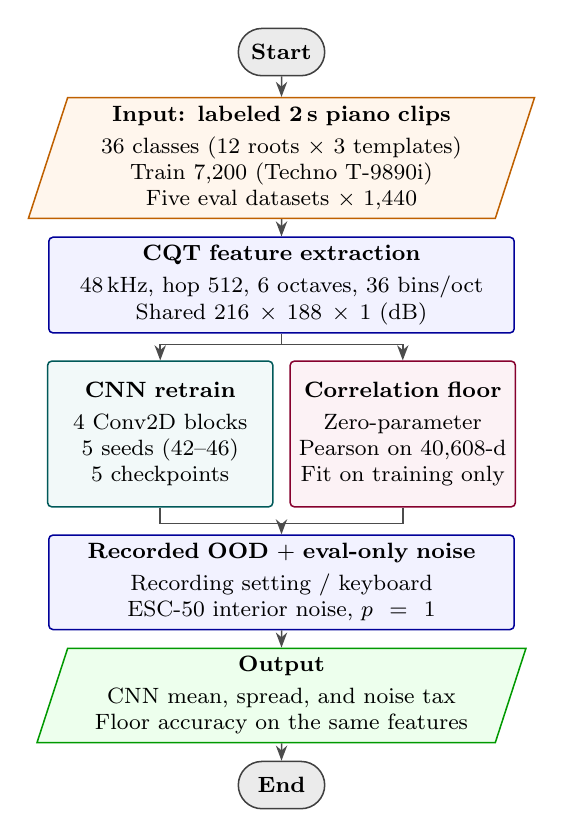
\begin{tikzpicture}[
    node distance=0.16cm and 0.10cm,
    >={Stealth},
    font=\footnotesize,
    base/.style={draw, align=center, minimum height=0.52cm, line width=0.55pt, inner sep=3pt},
    terminal/.style={base, shape=rounded rectangle, rounded rectangle arc length=180, draw=black!75, fill=black!8, minimum height=0.60cm, minimum width=1.8cm, inner xsep=10pt, inner ysep=2pt, font=\footnotesize\bfseries},
    process/.style={base, rectangle, rounded corners=1.5pt, draw=blue!60!black, fill=blue!5, text width=5.7cm},
    baseline/.style={base, rectangle, rounded corners=1.5pt, draw=purple!70!black, fill=purple!5, text width=2.65cm, minimum height=1.85cm},
    cnn/.style={base, rectangle, rounded corners=1.5pt, draw=teal!70!black, fill=teal!5, text width=2.65cm, minimum height=1.85cm},
    io/.style={base, trapezium, trapezium left angle=72, trapezium right angle=108, trapezium stretches body=true, draw=orange!75!black, fill=orange!7, text width=5.15cm, inner xsep=4pt},
    result/.style={base, trapezium, trapezium left angle=72, trapezium right angle=108, trapezium stretches body=true, draw=green!60!black, fill=green!7, text width=5.15cm, inner xsep=4pt},
    arrow/.style={->, line width=0.55pt, black!70}
  ]
    \node[terminal] (start) {Start};
    \node[io, below=0.26cm of start] (in1)
    {\textbf{Input: labeled 2\,s piano clips}\\[2pt]
     36 classes (12 roots $\times$ 3 templates)\\
     Train 7{,}200 (Techno T-9890i)\\
     Five eval datasets $\times$ 1{,}440};
    \node[process, below=0.22cm of in1] (p2)
    {\textbf{CQT feature extraction}\\[2pt]
     48\,kHz, hop 512, 6 octaves, 36 bins/oct\\
     Shared $216 \times 188 \times 1$ (dB)};
    \node[cnn, below left=0.34cm and 0.10cm of p2.south, anchor=north east] (cnn1)
    {\textbf{CNN retrain}\\[2pt]
     4 Conv2D blocks\\
     5 seeds (42--46)\\
     5 checkpoints};
    \node[baseline, below right=0.34cm and 0.10cm of p2.south, anchor=north west] (base1)
    {\textbf{Correlation floor}\\[2pt]
     Zero-parameter\\
     Pearson on 40{,}608-d\\
     Fit on training only};
    \node[process, below=0.34cm of $(cnn1.south)!0.5!(base1.south)$, anchor=north] (p5)
    {\textbf{Recorded OOD $+$ eval-only noise}\\[2pt]
     Recording setting / keyboard\\
     ESC-50 interior noise, $p=1$};
    \node[result, below=0.22cm of p5] (out)
    {\textbf{Output}\\[2pt]
     CNN mean, spread, and noise tax\\
     Floor accuracy on the same features};
    \node[terminal, below=0.22cm of out] (endn) {End};
    \draw[arrow] (start) -- (in1);
    \draw[arrow] (in1) -- (p2);
    \draw[arrow] (p2.south) -- ++(0,-0.14) -| (cnn1.north);
    \draw[arrow] (p2.south) -- ++(0,-0.14) -| (base1.north);
    \coordinate (merge) at ($(p5.north)+(0,0.14)$);
    \draw[line width=0.55pt, black!70] (cnn1.south) |- (merge);
    \draw[line width=0.55pt, black!70] (base1.south) |- (merge);
    \draw[arrow] (merge) -- (p5.north);
    \draw[arrow] (p5) -- (out);
    \draw[arrow] (out) -- (endn);
  \end{tikzpicture}%
  }
  \caption{Experimental pipeline. Shared CQT features feed a 5-seed CNN retrain and a correlation nearest-centroid floor. Overlays hit evaluation datasets only; CNN weights stay frozen after training.}
  \label{fig:methodology}
\end{figure}

\subsection{Two evaluation scenarios}\label{subsec3_0}

Scenario~1 (in-domain) holds instrument, room, and recording setting fixed and asks whether the CQT space separates the 36 classes at all. Five-fold cross-validation on the 7{,}200 Techno takes measures this.

Scenario~2 changes one factor at a time and tests each trained CNN checkpoint with no fine-tuning. Three recording-setting-shift datasets keep the Techno T-9890i and change the recording setup -- microphone, placement, and on-device signal chain, not the transducer alone (ThinkPad P14s Gen 2 Intel internal mic, Vivo Y27s phone, ASUS ROG Flow X13 2022 internal mic). Two keyboard-shift datasets then swap the instrument to a Yamaha PSR-S910 while reusing the ThinkPad and Flow recording setups already measured on the Techno. That pairing is the point: \texttt{thinkpad} versus \texttt{thinkpad-2} differs by keyboard, not by recording setup; \texttt{flow} versus \texttt{flow-2} does the same. \texttt{vivo} has no Yamaha counterpart, so it contributes recording-setting-shift evidence but not a matched pair. Table~\ref{tab:scenarios} lists every dataset. Eval-only noise (Section~\ref{subsec3_7}) hits all five 1{,}440-sample datasets. No checkpoint is fine-tuned on evaluation data.

\begin{table*}[t]
\caption{Recorded evaluation datasets. The CNN is trained on \texttt{training} and evaluated on every dataset. $^\dagger$\texttt{vivo} has no Yamaha counterpart.}\label{tab:scenarios}
\begin{tabular*}{\textwidth}{@{\extracolsep{\fill}}lllll@{}}
\toprule
Dataset & $N$ & Primary shift & Instrument & Recording setting \\
\midrule
\texttt{training} & 7{,}200 & None (in-domain) & Techno T-9890i & Xiaomi Redmi Pad 2 \\
\texttt{thinkpad} & 1{,}440 & Recording setting & Techno T-9890i & ThinkPad P14s Gen 2 (Intel) \\
\texttt{vivo} & 1{,}440 & Recording setting$^\dagger$ & Techno T-9890i & Vivo Y27s \\
\texttt{flow} & 1{,}440 & Recording setting & Techno T-9890i & ASUS ROG Flow X13 (2022) \\
\texttt{thinkpad-2} & 1{,}440 & Keyboard & Yamaha PSR-S910 & ThinkPad P14s Gen 2 (Intel) \\
\texttt{flow-2} & 1{,}440 & Keyboard & Yamaha PSR-S910 & ASUS ROG Flow X13 (2022) \\
\bottomrule
\end{tabular*}
\end{table*}

\subsection{Dataset acquisition}\label{subsec3_1}

A web recorder sends simultaneous MIDI note-on events over USB and captures the microphone. That removes manual playing errors and keeps the instrument's physical resonance and synthesis. The same trigger list and voicing are used for every dataset, so class identity does not change with the acoustic condition.

The vocabulary is 36 classes. Each class is a three-note piano sound: one of 12 roots (C, C$\sharp$, \ldots, B) times one of three interval templates (maj $+4,+3$; min $+3,+4$; dim $+3,+3$ semitones). A semitone is one chromatic step and occupies three CQT bins. Figures write \emph{C maj}, \emph{E dim}; file names keep the fourth-octave suffix. All takes sit in that octave, inside C1--C7 ($\approx$33--2093\,Hz) \cite{Telila2023}\cite{Harte2010}. The dim template places its three notes closer together than maj or min \cite{Byambatsogt2020}. Both instruments use a grand-piano preset; they still differ in sample set, loudspeaker, and cabinet.

\begin{enumerate}[1.]
\item \textbf{Training (\texttt{training})}: 200 samples per class, 7{,}200 total. Xiaomi Redmi Pad 2 mic, Techno T-9890i Acoustic Grand Piano. Attack delays 0--150\,ms approximate keystroke asynchrony \cite{Bella2011}. OGG/OPUS, 48{,}000\,Hz, 32-bit, mono, no filters. Sixteen clips (8\% of $C$ diminished, a recorder fault) are digital silence; they remain in the training set used here.
\item \textbf{Recording-setting shift (\texttt{thinkpad}, \texttt{vivo}, \texttt{flow})}: 40 per class, 1{,}440 each, WAV. Techno T-9890i on the ThinkPad P14s Gen 2 (Intel) internal mic, a Vivo Y27s phone mic, and the ASUS ROG Flow X13 (2022) internal mic.
\item \textbf{Keyboard shift (\texttt{thinkpad-2}, \texttt{flow-2})}: 40 per class, 1{,}440 each, WAV. Yamaha PSR-S910 on the ThinkPad and Flow recording setups already used on the Techno.
\end{enumerate}

No evaluation clip enters training, validation, early stopping, or hyperparameter choice.

\subsection{CQT feature extraction}\label{subsec3_2}

We compute CQT with \texttt{librosa.cqt()}. Each bin $f_k$ has constant quality
\begin{equation}
Q = \frac{f_k}{f_{k+1} - f_k} = \frac{1}{2^{1/B} - 1}
\label{eq:cqt}
\end{equation}
where $B$ is bins per octave \cite{Li2021}\cite{Lacoste2007}. Logarithmic spacing lines bins up with semitones, so a transposition is a vertical shift and a major third is the same bin distance on every root \cite{Harte2010}.

Table~\ref{tab:cqt-extraction-params} lists parameters. Thirty-six bins per octave (3 per semitone) resolve major ($+4,+3$), minor ($+3,+4$), and diminished ($+3,+3$) intervals \cite{Akram2025}\cite{OHanlon2021}. Each clip is truncated to a fixed 2.0\,s. Equation~\ref{eq:frames} gives 188 frames and a uniform shape $216 \times 188 \times 1$. Magnitudes go to dB with \texttt{librosa.amplitude\_to\_db(..., ref=np.max)}. The same parameters are used for training, every recorded dataset, and the noise overlay.

\begin{equation}
\text{frames} = \frac{\text{duration} \times \text{sample rate}}{\text{hop size}}
\label{eq:frames}
\end{equation}

\begin{table}[t]
\caption{CQT feature extraction parameters}\label{tab:cqt-extraction-params}
\begin{tabular}{@{}ll@{}}
\toprule
Parameter & Value \\
\midrule
Sample rate & 48{,}000\,Hz \\
Hop size & 512 samples \\
Octaves & 6 \\
Bins per octave & 36 \\
Total bins & 216 \\
Frequency range & C1 (32.70\,Hz) to C7 (2{,}093\,Hz) \\
Window & Hann \\
Frame length & 188 \\
Output shape & $216 \times 188 \times 1$ \\
\bottomrule
\end{tabular}
\end{table}

\begin{figure}[t]
\centering
\includegraphics[width=\columnwidth]{fig-cqt-train.png}
\caption{Training CQT of C maj ($+4,+3$) and C min ($+3,+4$): same root, one-semitone gap in the middle note. Frequency in Hz.}
\label{fig:cqt-spectrograms}
\end{figure}

\subsection{CNN architecture and training}\label{subsec3_3}

The CNN follows Wolf-Monheim \cite{Wolf-Monheim2025}, originally designed for environmental sound classification on ESC-50. Its compact four-block convolutional structure without recurrent layers or attention is appropriate for fixed-window classification from static spectrograms.

Table~\ref{tab:cnn-architecture} lists layers. Input batch normalization fits its scale and shift to the training distribution once and applies that fixed transform to every clip at inference. The four Conv2D--MaxPooling2D blocks build a progressive hierarchy: the first block (64 filters) captures low-level spectral texture; the second (128 filters) encodes mid-level harmonic interval patterns; the third and fourth (256 filters each) represent chord-quality abstractions. The $3\times3$ receptive field matches the 1--2 bin frequency shifts that distinguish chord types, while MaxPooling provides spatial subsampling and limited translation invariance \cite{Purwono2022}. Dropout (rate 0.5) limits co-adaptation to the Techno piano voice.

\begin{table}[t]
\caption{CNN architecture specification}\label{tab:cnn-architecture}
\begin{tabularx}{\columnwidth}{@{}lXl@{}}
\toprule
Layer & Output shape & Notes \\
\midrule
BatchNorm & $216{\times}188{\times}1$ & Input normalization \\
Conv2D & $216{\times}188{\times}64$ & $3{\times}3$, ReLU, same \\
MaxPool & $108{\times}94{\times}64$ & $2{\times}2$, stride 2 \\
Conv2D & $108{\times}94{\times}128$ & $3{\times}3$, ReLU, same \\
MaxPool & $54{\times}47{\times}128$ & $2{\times}2$, stride 2 \\
Conv2D & $54{\times}47{\times}256$ & $3{\times}3$, ReLU, same \\
MaxPool & $27{\times}23{\times}256$ & $2{\times}2$, stride 2 \\
Conv2D & $27{\times}23{\times}256$ & $3{\times}3$, ReLU, same \\
MaxPool & $13{\times}11{\times}256$ & $2{\times}2$, stride 2 \\
Flatten & 36{,}608 & \\
Dense & 256 & ReLU \\
Dropout & 256 & rate 0.5 \\
Dense & 36 & Softmax \\
\bottomrule
\end{tabularx}
\end{table}

Training follows Table~\ref{tab:cnn-training-config}. Stratified 80/10/10 sampling keeps class balance. The seed is reused for the split, the weight initialization, and TensorFlow's global RNG. \texttt{ReduceLROnPlateau} multiplies the learning rate by 0.1 after 2 stagnant val-loss epochs; \texttt{EarlyStopping} stops after 6; max 50 epochs \cite{Wolf-Monheim2025}. The 10\% test split is held out of training and validation. This configuration is retrained from five seeds (42--46). Table~\ref{tab:cnn-training-config}'s seed value is the reference used for seed 42 of the retrain batch.

\begin{table}[t]
\caption{CNN training configuration}\label{tab:cnn-training-config}
\begin{tabular}{@{}ll@{}}
\toprule
Parameter & Value \\
\midrule
Seeds & 42, 43, 44, 45, 46 \\
Train / Val / Test split & 80\% / 10\% / 10\% \\
Batch size & 32 \\
Initial learning rate & 0.001 \\
Optimizer & Adam \\
Weight initialization & Glorot uniform \\
Loss & Categorical cross-entropy \\
Max epochs & 50 \\
EarlyStopping patience & 6 epochs \\
ReduceLROnPlateau & factor 0.1, patience 2 \\
\bottomrule
\end{tabular}
\end{table}

\subsection{5-fold cross-validation}\label{subsec3_5}

Five folds on all 7{,}200 training samples, 80/20 per fold, measure in-domain score independent of one train/test split. Each fold retrains the CNN from a fresh random initialization and a fixed per-fold seed. Fold test partitions never enter training or early stopping for that fold.

\subsection{Correlation nearest-centroid floor}\label{subsec3_baseline}

A zero-parameter classifier is scored on the identical CQT features as a deterministic floor. Each class centroid is the mean of its flattened training CQT matrices ($216\times188 \to 40{,}608$), excluding the sixteen silent clips. A test clip is compared to all 36 centroids by Pearson correlation (both mean-centered and unit-normalized, then cosine similarity), so a uniform per-clip gain or offset in dB does not change the ranking. The classifier needs no gradient step, validation split, or seed. It is not a proposed chord-recognition system; it asks only whether the true class still ranks first among 36 after the shift.

\subsection{Eval-only noise}\label{subsec3_7}

Additive interior noise hits already out-of-domain datasets without retraining, applied to all five CNN checkpoints and to the floor. ESC-50 interior/domestic clips \cite{Piczak2015} are converted to CQT with the same hop and binning as the chord features, yielding a 400-clip bank over 10 classes. Mixing is performed in the CQT power domain at a uniform SNR drawn from $[10, 25]$\,dB (realized mean 17.5\,dB) with a random time roll. Overlay probability is 1 (every evaluation sample is degraded), the draw is random per sample with a fixed seed, and wet features are not written back into the training tree. This is a controlled interior overlay, not a claim that ESC-50 matches any one room. Indoor room impulse responses and measured microphone impulse responses were applied under the same eval-only rule; they are not reported as primary results here.

\subsection{Evaluation metrics}\label{subsec3_6}

Accuracy, precision, recall, and F1 come from the confusion matrix. For a one-versus-rest partition of a single class the counts are True Positives (TP), True Negatives (TN), False Positives (FP), and False Negatives (FN):
\begin{equation}
\mathrm{P}=\frac{\mathrm{TP}}{\mathrm{TP}+\mathrm{FP}},\quad
\mathrm{R}=\frac{\mathrm{TP}}{\mathrm{TP}+\mathrm{FN}},\quad
\mathrm{F1}=\frac{2\mathrm{PR}}{\mathrm{P}+\mathrm{R}}.
\label{eq:prf}
\end{equation}
Accuracy is the fraction of clips with the correct label. Macro P, R, and F1 are unweighted means over the 36 classes. We report accuracy as the headline metric and give the CNN as mean $\pm$ standard deviation over the five seeds, with the min--max range where the spread is the finding.

\section{Results}\label{sec4}

\subsection{CQT feature extraction}\label{subsec4_1}

Every clip becomes a $216 \times 188$ CQT dB matrix. Fig.~\ref{fig:cqt-spectrograms} shows C maj and C min from the training set: same root, one semitone (three CQT bins) in the middle note.

\subsection{In-domain performance}\label{subsec4_2}

Under Scenario~1 the CNN scores 1.00 accuracy, precision, recall, and F1 on every fold of the 7{,}200 Techno takes, and on the held-out test split of every one of the five retrains ($1.000\pm0.000$). Resubstitution on the full training dataset is 0.9999: one $C$ diminished clip is predicted $C$ minor. With instrument, room, and recording setting fixed, the CQT space separates all 36 classes for every seed. That result certifies separability, not OOD behavior.

The correlation floor's own 5-fold in-domain accuracy on the 7{,}184 non-silent clips is $0.9996\pm0.0006$, below its 1.000 on every held-out recording. The five held-out datasets are not an easier case than the training pool's own held-out fold.

\subsection{Recorded out-of-domain evaluation}\label{subsec4_3}

Table~\ref{tab:cross-domain} and Fig.~\ref{fig:cross-domain} score the five CNN checkpoints and the correlation floor on the five held-out recordings. The floor reaches 1.000 on every dataset, recording-setting shift and keyboard shift alike.

The CNN's mean follows the factor that changed. Recording-setting shift (Techno, new microphone) stays high: $0.961\pm0.040$ on \texttt{thinkpad}, $0.903\pm0.085$ on \texttt{vivo}, $0.911\pm0.078$ on \texttt{flow}. Keyboard shift (Yamaha on a microphone already scored on the Techno) is lower: $0.803\pm0.106$ on \texttt{thinkpad-2}, $0.815\pm0.096$ on \texttt{flow-2}. On the mean, swapping the keyboard costs more than swapping the recording setup.

A single seed does not report that mean. On \texttt{thinkpad-2} the five CNN runs span 0.705--0.963; on \texttt{flow-2} they span 0.720--0.961. That interval is wider than the gap between the recording-setting means and the keyboard means. A published keyboard-shift cost taken from one run sits inside the seed spread, not at an edge of it. Every one of those runs still scores 1.00 in-domain.

\begin{table}[htbp]
\caption{Out-of-domain accuracy. Floor: correlation nearest-centroid, fit once on the 7{,}184 non-silent training clips. CNN: mean, standard deviation, and range over 5 seeds.}\label{tab:cross-domain}
\setlength{\tabcolsep}{3.5pt}
\begin{tabular}{@{}lcccc@{}}
\toprule
Dataset & Floor & CNN mean & sd & min--max \\
\midrule
\texttt{thinkpad} & 1.000 & 0.961 & 0.040 & 0.895--0.999 \\
\texttt{vivo} & 1.000 & 0.903 & 0.085 & 0.776--0.999 \\
\texttt{flow} & 1.000 & 0.911 & 0.078 & 0.801--0.994 \\
\texttt{thinkpad-2} & 1.000 & 0.803 & 0.106 & 0.705--0.963 \\
\texttt{flow-2} & 1.000 & 0.815 & 0.096 & 0.720--0.961 \\
\bottomrule
\end{tabular}
\end{table}

\begin{figure}[htbp]
\centering
\includegraphics[width=\columnwidth,height=0.28\textheight,keepaspectratio]{fig-cross-domain.pdf}
\caption{Out-of-domain accuracy on the five held-out recordings. The series discussed in the text are the correlation floor and the CNN mean $\pm$ sd over 5 seeds.}
\label{fig:cross-domain}
\end{figure}

\subsection{Eval-only noise}\label{subsec4_4}

Table~\ref{tab:noise} and Fig.~\ref{fig:aug} score the same five CNN checkpoints and the same floor after ESC-50 interior noise is mixed into every evaluation clip. The floor is effectively unaffected (0.999 on \texttt{thinkpad}, 1.000 elsewhere). The CNN is not. Mean accuracy under noise is 0.827--0.858 on the three Techno datasets and 0.650--0.670 on the two Yamaha datasets: a drop of 6.5--10.2 points from each Techno recorded mean and 14.5--15.3 points from each Yamaha recorded mean. Noise compounds keyboard shift rather than substituting for it. Pooled across datasets and seeds, CNN noise accuracy is 0.770.

\begin{table}[htbp]
\caption{CNN accuracy before and after eval-only ESC-50 noise, mean over 5 seeds. Tax is recorded mean minus noise mean, in percentage points. Floor accuracy under the same noise is 0.999--1.000.}\label{tab:noise}
\setlength{\tabcolsep}{3.5pt}
\begin{tabular}{@{}lccc@{}}
\toprule
Dataset & Recorded & Noise & Tax \\
\midrule
\texttt{thinkpad} & 0.961 & 0.858 & 10.2 \\
\texttt{vivo} & 0.903 & 0.827 & 7.6 \\
\texttt{flow} & 0.911 & 0.846 & 6.5 \\
\texttt{thinkpad-2} & 0.803 & 0.650 & 15.3 \\
\texttt{flow-2} & 0.815 & 0.670 & 14.5 \\
\bottomrule
\end{tabular}
\end{table}

\begin{figure}[htbp]
\centering
\includegraphics[width=\columnwidth,height=0.28\textheight,keepaspectratio]{fig-aug-compare.pdf}
\caption{Accuracy under eval-only overlays, pooled over seeds. The text reports the noise column; RIR and DIR were collected under the same protocol.}
\label{fig:aug}
\end{figure}

\section{Discussion}\label{sec5}

\subsection{What the CNN measures}\label{subsec5_0}

The CNN learns the 36-way task when the keyboard, room, and recording setting stay fixed. That is the in-domain result, and it is stable across folds and across the five retrains. The OOD result is a different object. On the mean, a new microphone on the Techno is cheaper than a new keyboard on a microphone already measured; eval-only interior noise then costs more on the Yamaha recordings than on the Techno ones. Those two orderings are the factorized reading this protocol was built to produce.

They are orderings of a mean. The seed range on either Yamaha dataset is large enough that one run can look like near-free keyboard shift (0.96) and another like a 30-point drop (0.70), with in-domain accuracy 1.00 in both cases. A single-run domain-shift cost on this task reports where that seed's optimizer landed as much as it reports the acoustic factor.

\subsection{The classes do not merge}\label{subsec5_1}

The correlation floor reaches 1.000 on every held-out recording and stays at 0.999--1.000 under the same noise. Pearson matching on flattened CQT, after per-clip mean-centering and unit-normalization, still ranks the true class first among 36. The vocabulary is therefore still linearly separable in the representation the CNN is given. The CNN's OOD misses are failures of a trained instance under a global envelope the floor removes by construction, not evidence that major, minor, and diminished templates become the same object after a mic or keyboard change.

That is the only use of the floor in this paper. MIDI-triggered isolated triads with one fixed voicing are a protocol on which a template match can saturate. The same classifier is not a claim about songs, expressive timing, or a wider harmonic vocabulary.

\subsection{Relation to prior OOD piano work}\label{subsec5_2}

Edwards et al.\ \cite{Edwards2024} applied test-time noise and reverb to a clean-trained transcription model and saw drops of several to about 19 note-onset F1 points on MAPS, then recovered the OOD set with train-time mixing. Our noise tax, 6.5--15.3 accuracy points depending on the dataset, sits in a comparable range despite a different task and metric. We withheld train-time mixing so the recorded numbers stay a factorized reading of a fixed CQT--CNN. Mixing is the natural next intervention; any later claim that it closed the gap should be checked against the five-seed spread and against the floor, not only against in-domain 1.00 and one run.

\subsection{Limitations}\label{subsec5_3}

Both instruments are digital pianos on a grand-piano preset; an acoustic grand would be a larger keyboard factor. All voicings are isolated fourth-octave triads, and training uses one tablet microphone. \texttt{vivo} has no keyboard-shift counterpart. Sixteen silent training clips went undetected by resubstitution accuracy; they remain in the set used here. No recorded dataset covers environmental shift directly; the noise overlay is a controlled proxy, not a recorded room. Five seeds establish that a single run is unstable; they are a thin sample of the training distribution. A larger retrain batch that also varied input normalization and dropped the silent clips is not part of this report.

\section{Conclusion}\label{sec6}

A compact CQT--CNN recognizes 36 isolated piano triads at 1.00 in-domain, on every fold and every one of five retrains. Under a factorized recording-setting and keyboard shift the same checkpoints do not agree: mean accuracy stays higher when only the microphone changes (0.903--0.961) than when the keyboard changes on a matched recording setup (0.803--0.815), and individual Yamaha runs span 0.705--0.963. Eval-only interior noise then compounds the keyboard cost. A correlation nearest-centroid classifier on the same features remains at 1.000 on every recorded set, so the classes stay separable and the OOD misses belong to the trained CNN. Future claims about this protocol should report a seed spread, and should check a deterministic floor, before treating one run's OOD number as the cost of the shift.

\backmatter

\bmhead{Author contributions}
All authors contributed to study conceptualization and design. Material preparation, data acquisition, experimentation, analysis, and drafting were performed by CGS. All authors reviewed and approved the final version.

\bmhead{Funding}
No funding was received for this work.

\bmhead{Data availability}
The piano chord dataset is publicly available at \url{https://zenodo.org/records/21077144}.

\bmhead{Code availability}
The dataset generation and recording tool is available at \url{https://github.com/sglkc/chords-dataset-generator/}. Experiment notebooks are available in the project repository.

\section*{Declarations}

\bmhead{Conflict of interest}
The authors declare no competing interests.

\bmhead{Ethics approval}
Not applicable.

\bmhead{Consent for publication}
All authors approved the final manuscript.

\bibliography{mendeley}

\end{document}
